\section{РАЗРАБОТКА БАЗЫ ДАННЫХ}
\subsection{Концептуальная модель}

\textbf{Предметная область} - совокупность объектов,
свойства которых и отношения между которыми рассматриваются в рамках некоторого исследования.

\textbf{Модель предметной области} - некоторая система, адекватно имитирующая
структуру и функционирование исследуемой предметной области.

\textbf{Концептуальная модель} - это структура моделируемой предметной области,
свойств её элементов и причинно-следственных связей, присущих системе и
существенных для достижения цели моделирования.
В рамках этапа концептуального моделирования выделяются основные смысловые единицы (сущности)
предметной области, определяются и описываются связи между ними.

Концептуальная модель ориентирована на потенциальных пользователей базы данных,
так как представляет предметную область на их уровне понимания.
Этот уровень называется системно-независимым или предметно-ориентированным.

Основные символы модели данных в ARIS Express 2.4i \cite{ArisExpress} 
изображены на рисунке~\ref{fig:ArisDataModel}.

\begin{figure}[!h]
    \centering

    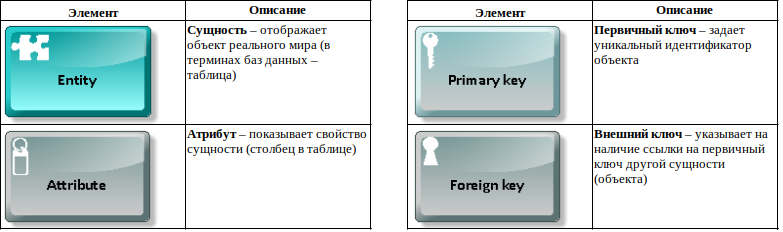
\includegraphics[height=13cm]
    {assets/ARIS/DataModel/Elements/ArisDataModel.png}

    \caption{Основные символы модели данных (ARIS Express 2.4i Data Model)}

    \label{fig:ArisDataModel}
\end{figure}

Модель данных позволяет взглянуть на данные (например, бизнес-объекты) и отношения между ними.

Виды отношений между объектами (1:1, 1:n, ...) задаются с помощью атрибутов связей.

Виды связей сущностей в ARIS Express 2.4i \cite{ArisExpress} Data Model изображены на рисунке~\ref{fig:ArisDataModelRelations}.

\begin{figure}[!h]
    \centering

    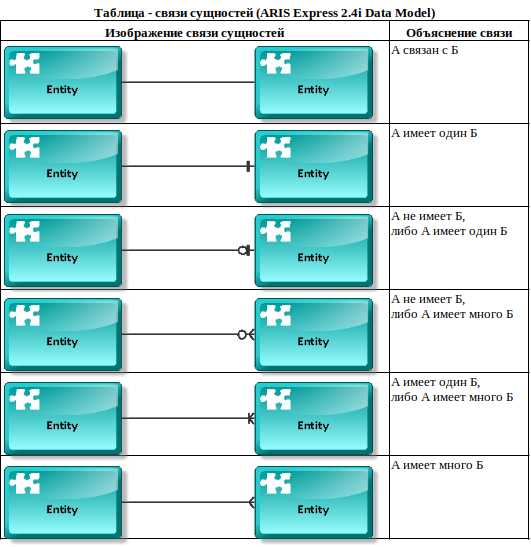
\includegraphics[width=16cm]
    {assets/ARIS/DataModel/Relations/ArisDataModelRelations.png}

    \caption{Связи сущностей (ARIS Express 2.4i Data Model)}

    \label{fig:ArisDataModelRelations}
\end{figure}

В ARIS Express 2.4i \cite{ArisExpress} Data Model существуют следующие виды связей сущностей:
\begin{itemize}
    \item к одному;
    \item нет связи или к одному;
    \item нет связи или ко многим;
    \item к одному или ко многим;
    \item ко многим.
\end{itemize}

\newpage

\subsubsection{ЛКМ для процедуры <<Создание инвентаризационной комиссии>>}

Локальная концептуальная модель
(спроектированна с использованием ARIS Express 2.4 \cite{ArisExpress} Data Model)
для процедуры <<Создание инвентаризационной комиссии>>
изображена на рисунке~\ref{fig:DE_DOC_OrderCreationInventoryCommission}.

Локальная концептуальная модель соотвествует функциональному дереву ОА <<Косметический салон>>.

\begin{figure}[!h]
    \centering

    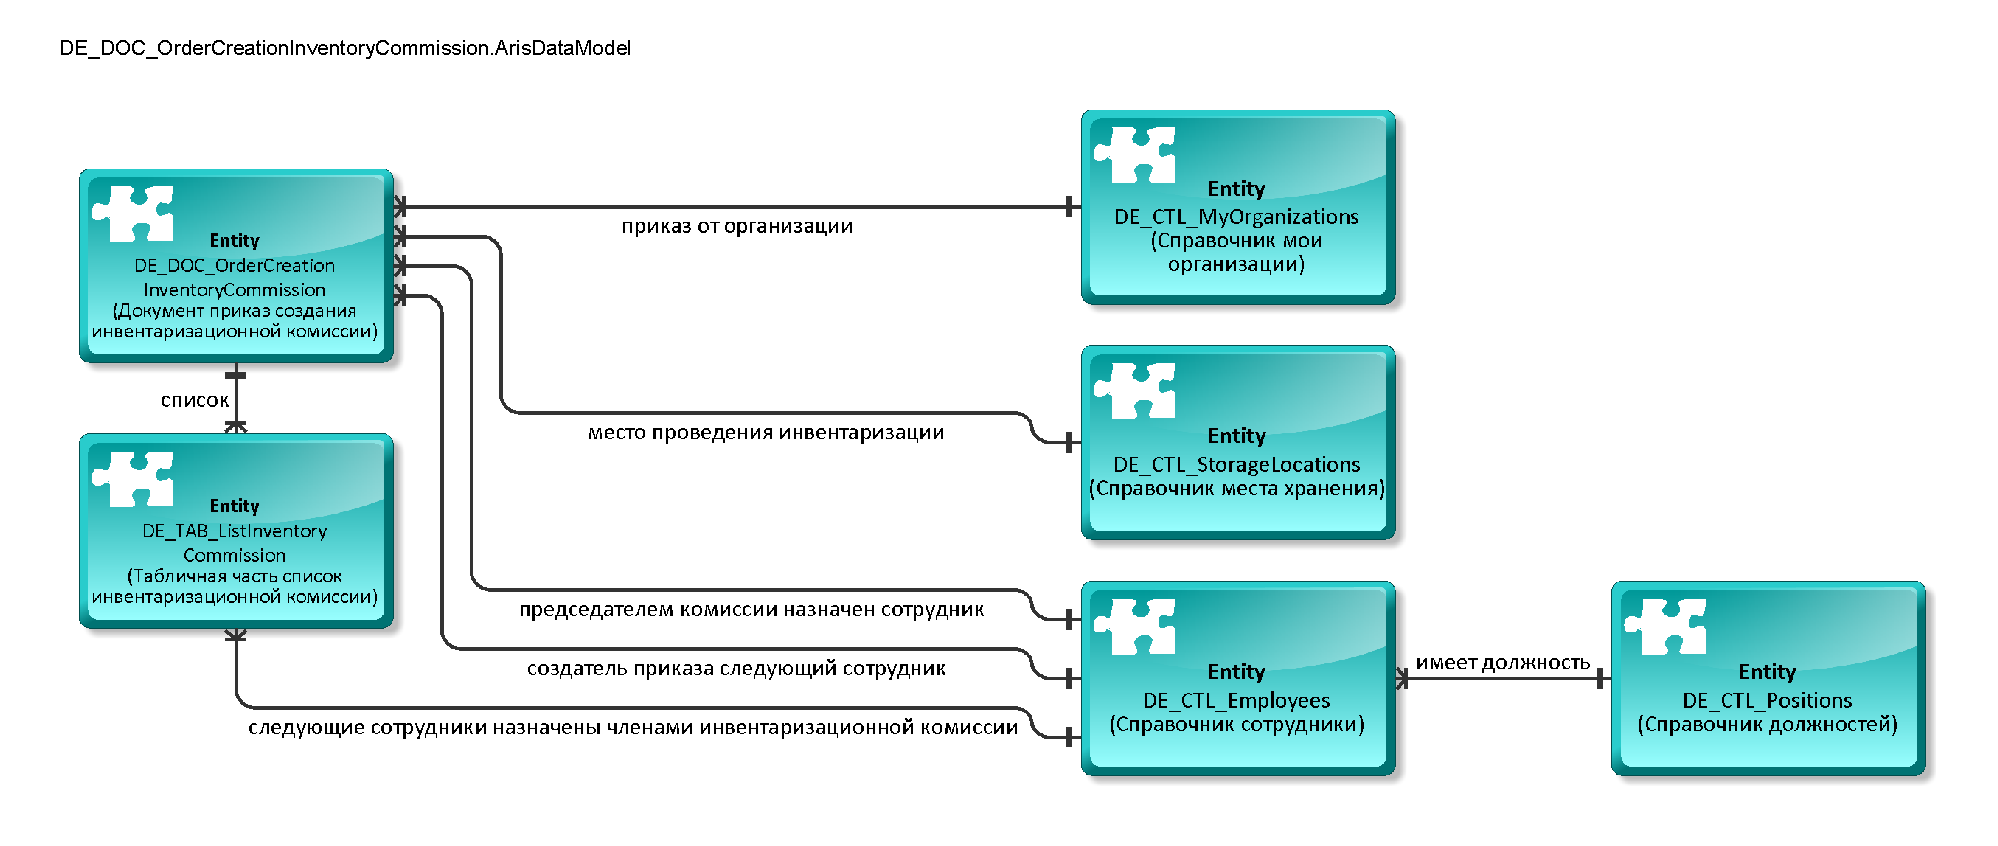
\includegraphics[width=15cm]
    {assets/ARIS/DataModel/ConceptualModels/DE_DOC_OrderCreationInventoryCommission.ArisDataModel.pdf}

    \caption{ЛКМ для процедуры <<Создание инвентаризационной комиссии>>}

    \label{fig:DE_DOC_OrderCreationInventoryCommission}
\end{figure}

% \begin{figure}[!h]
%     \centering

%     \includegraphics[width=18cm]
%     {assets/database/DataModel_DOC_PrikazCozdInventKom.adf.pdf}

%     \caption{Локальная концептуальная модель для бизнес процесса с документом <<Приказ о создании инвентаризационной комиссии>>}

%     \label{fig:DataModel_DOC_PrikazCozdInventKom}
% \end{figure}

%\newpage

\subsubsection{ЛКМ для процедуры <<Проведение инвентаризации>>}

Локальная концептуальная модель
(спроектированна с использованием ARIS Express 2.4 \cite{ArisExpress} Data Model)
для процесса с документом <<Проведение инвентаризации>>
изображена на рисунке~\ref{fig:DE_DOC_InventoryList}.

Локальная концептуальная модель соотвествует функциональному дереву ОА <<Косметический салон>>.

\begin{figure}[!h]
    \centering

    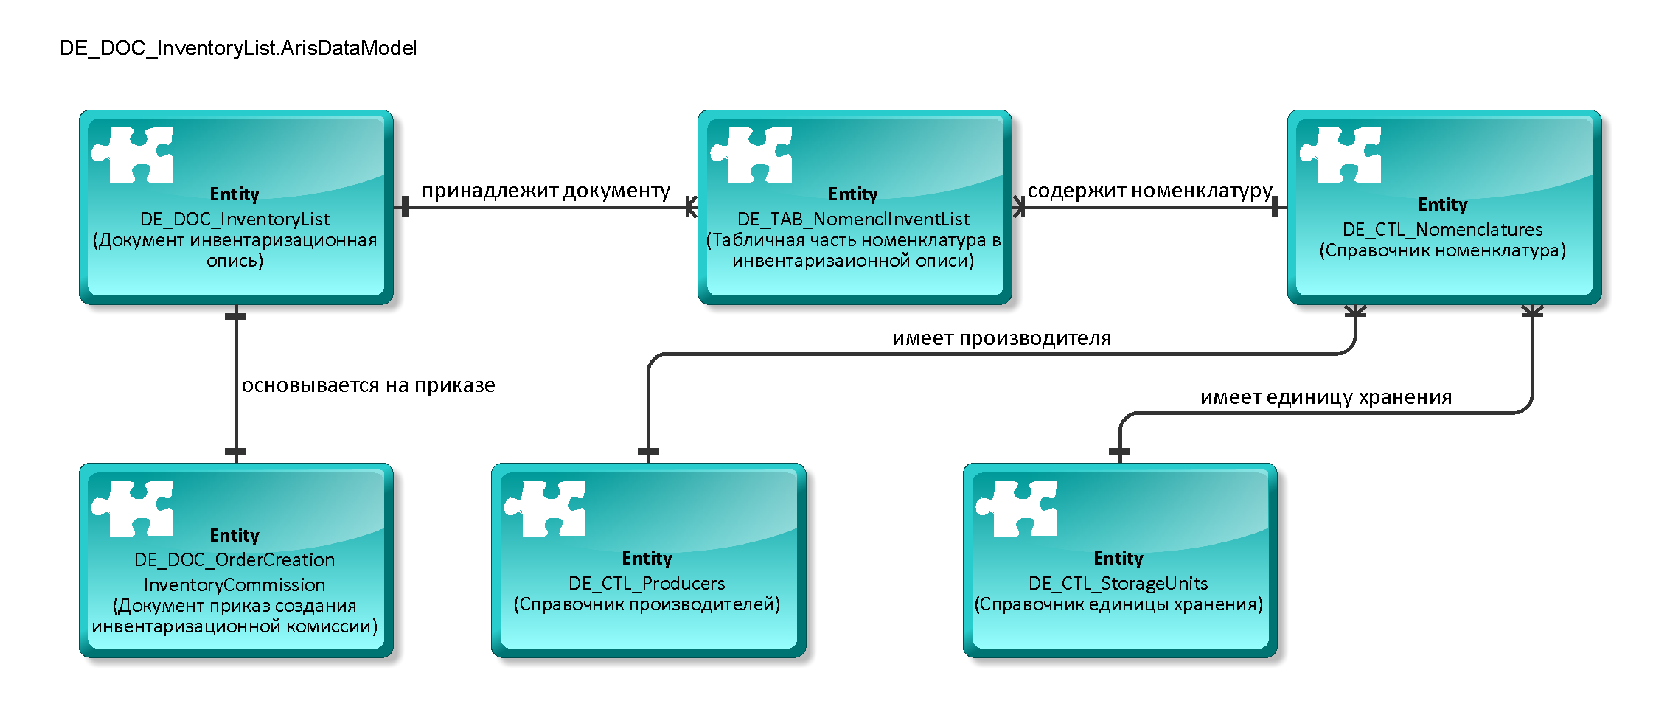
\includegraphics[width=15cm]
    {assets/ARIS/DataModel/ConceptualModels/DE_DOC_InventoryList.ArisDataModel.pdf}

    \caption{ЛКМ для процедуры <<Создание инвентаризационной комиссии>>}

    \label{fig:DE_DOC_InventoryList}
\end{figure}

% \begin{figure}[!h]
%     \centering
% 
%     \includegraphics[height=8cm]
%     {assets/database/DataModel_DOC_InventOpec'.adf.pdf}
% 
%     \caption{Локальная концептуальная модель для бизнес процесса с документом <<Инвентаризационная опись>>}
% 
%     \label{fig:DataModel_DOC_InventOpic}
% \end{figure}

% \newpage
\subsubsection{Общая концептуальная модель}

Концептуальная модель
(спроектированна с использованием ARIS Express 2.4 \cite{ArisExpress} Data Model)
состоит из локальных концептуальных моделей и
изображена на рисунке~\ref{fig:GeneralConceptualModel}.

\begin{figure}[!h]
    \centering

    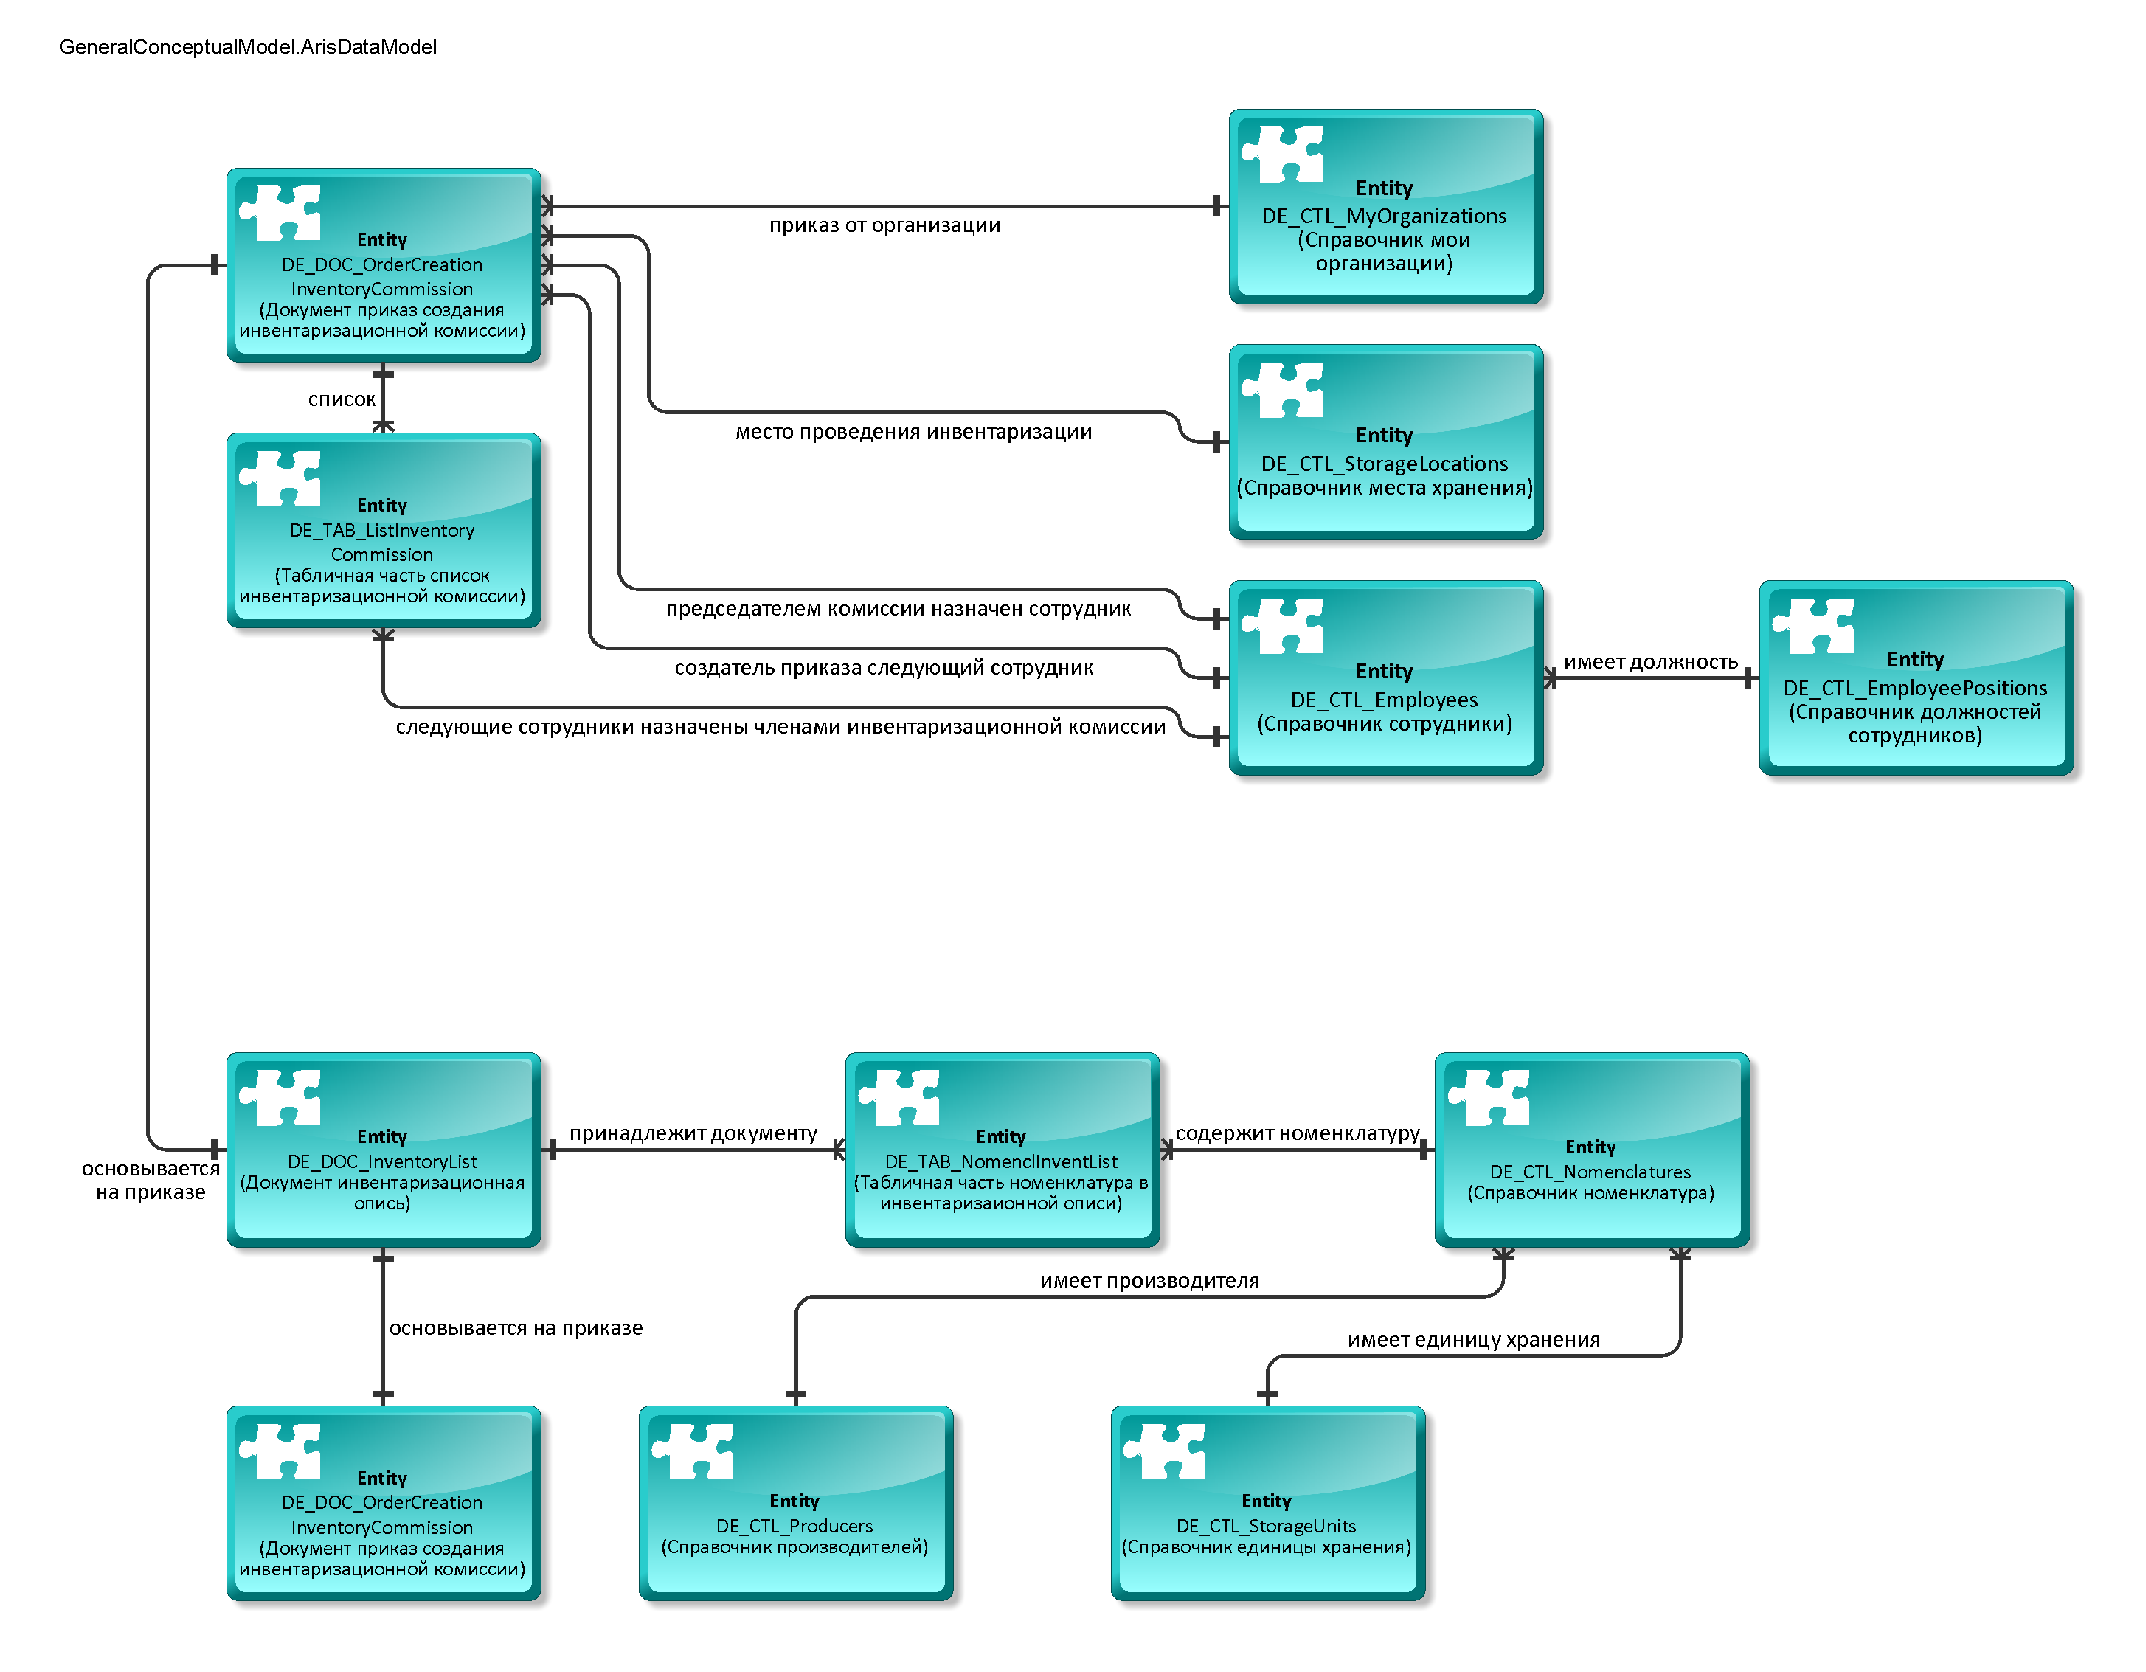
\includegraphics[width=16cm]
    {assets/ARIS/DataModel/GeneralConceptualModel/GeneralConceptualModel.ArisDataModel.pdf}

    \caption{Общая концептуальная модель}

    \label{fig:GeneralConceptualModel}
\end{figure}

% \begin{figure}[!h]
%     \centering
%     \includegraphics[height=8cm]
%         {assets/database/DataModel_DOC.bundle.adf.pdf}
%     \caption{Концептуальная модель}
%     \label{fig:DataModel_DOC}
% \end{figure}

\newpage
\subsection{Логическая модель}

\textbf{Логическая модель} - это модель данных конкретной предметной области,
представленной в виде таблиц и их связей.

Виды связей таблиц в SQL Power Architect 1.0.7 \cite{SqlPowerArhitect}
изображены на рисунке~\ref{fig:RelationsSqlPowerArchitect}

\begin{figure}[!h]
    \centering

    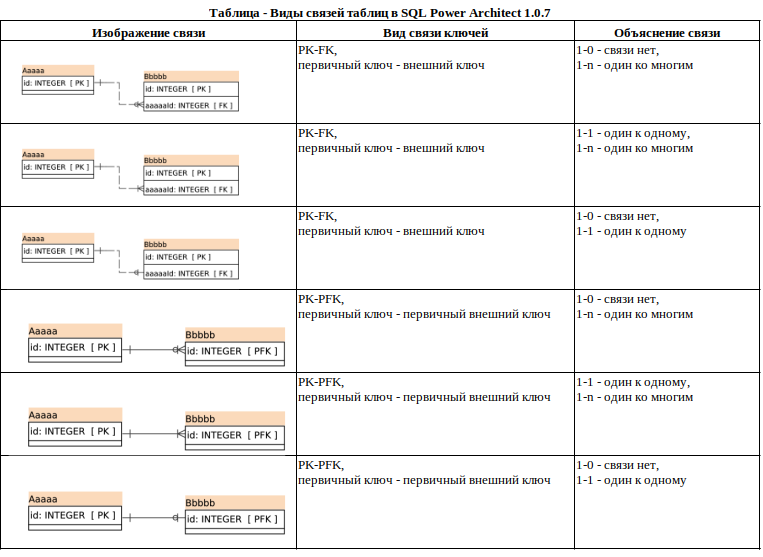
\includegraphics[width=18cm]
    {assets/database/Relations/RelationsSqlPowerArchitect.png}

    \caption{Виды связей таблиц в SQL Power Architect 1.0.7}

    \label{fig:RelationsSqlPowerArchitect}
\end{figure}

\textbf{Физическая модель} - это представление в виде SQL скриптов, которые создают таблицы и связи между ними,
которые получаются из логической модели.

\textbf{Первая нормальная форма} (1НФ) \cite{habr_1nf_6nf}.
Отношение находится в 1НФ, если все его атрибуты являются простыми,
все используемые домены должны содержать только скалярные значения.
Не должно быть повторений строк в таблице.

\textbf{Вторая нормальная форма} (2НФ) \cite{habr_1nf_6nf}.

Отношение находится во 2НФ, если оно находится в 1НФ и каждый не ключевой атрибут неприводимо зависит от Первичного Ключа (PK).

\textbf{Третья нормальная форма} (3НФ) \cite{habr_1nf_6nf}.

Отношение находится в 3НФ, когда находится во 2НФ и каждый не ключевой атрибут нетранзитивно зависит от первичного ключа.
Второе правило требует выносить все не ключевые поля, содержимое которых может относиться к нескольким записям таблицы в отдельные таблицы.

\textbf{Механизмы целостности} нужно для того, чтобы избежать ситуации не правильного заполнения базы данных.
Для атрибута выбирается тип данных, а у типа данных есть какой-то домен. Например, суть домена <<Код>> состоит в том,
что это целое число (тип INTEGER) и оно больше нуля (CHECK id > 0).
Также могут возникнуть ситуации, когда в базе данных не нужны, либо нужны те или иные атрибуты.
Для этого атрибуту можно присвоить NOT NULL, то есть атрибут важен для заполнения и не может быть пустым.
Когда атрибут не задан, то в базе данных он имеет значение NULL.
В базе данных можно предусмотреть DEFAULT-значения, например, если мы не задали дату,
то у нас отработает процедура NOW(), которая поставит текущую дату.

% = = = = = = = = = = = = = = = = = = = = = = = = = = = = = = = =

\subsubsection{Механизмы целостности для справочника <<Номенклатура>>}

Таблица с механизмами целостности изображена на рисунке~\ref{fig:Logic_DE_CTL_Nomenclatures}.

\begin{figure}[!h]
    \centering

    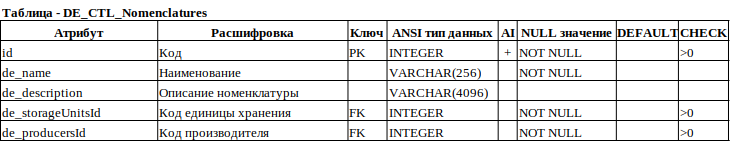
\includegraphics[width=18cm]
    {assets/database/Types/DE_CTL_Nomenclatures.png}

    \caption{Таблица DE\_CTL\_Nomenclatures}

    \label{fig:Logic_DE_CTL_Nomenclatures}
\end{figure}

% = = = = = = = = = = = = = = = = = = = = = = = = = = = = = = = =

\subsubsection{Механизмы целостности для справочника <<Сотрудники>>}

Таблица с механизмами целостности изображена на рисунке~\ref{fig:Logic_DE_CTL_Employees}.

\begin{figure}[!h]
    \centering

    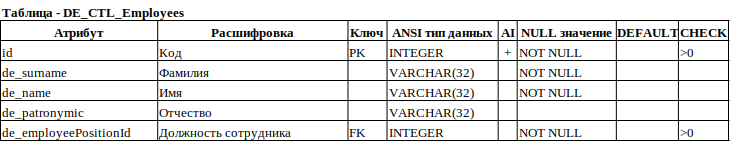
\includegraphics[width=18cm]
    {assets/database/Types/DE_CTL_Employees.png}

    \caption{Таблица DE\_CTL\_Employees}

    \label{fig:Logic_DE_CTL_Employees}
\end{figure}

% = = = = = = = = = = = = = = = = = = = = = = = = = = = = = = = =

\subsubsection{Механизмы целостности для справочника <<Должности>>}

Таблица с механизмами целостности изображена на рисунке~\ref{fig:Logic_DE_CTL_Positions}.

\begin{figure}[!h]
    \centering

    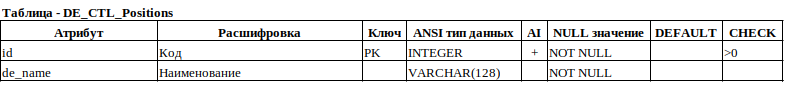
\includegraphics[width=18cm]
    {assets/database/Types/DE_CTL_Positions.png}

    \caption{Таблица DE\_CTL\_Positions}

    \label{fig:Logic_DE_CTL_Positions}
\end{figure}

% = = = = = = = = = = = = = = = = = = = = = = = = = = = = = = = =

\subsubsection{Механизмы целостности для справочника <<Единицы хранения>>}

Таблица с механизмами целостности изображена на рисунке~\ref{fig:Logic_DE_CTL_StorageUnits}.

\begin{figure}[!h]
    \centering

    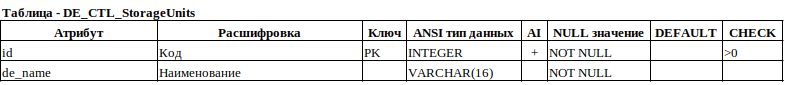
\includegraphics[width=18cm]
    {assets/database/Types/DE_CTL_StorageUnits.png}

    \caption{Таблица DE\_CTL\_StorageUnits}

    \label{fig:Logic_DE_CTL_StorageUnits}
\end{figure}

% = = = = = = = = = = = = = = = = = = = = = = = = = = = = = = = =

\subsubsection{Механизмы целостности для справочника <<Мои организации>>}

Таблица с механизмами целостности изображена на рисунке~\ref{fig:Logic_DE_CTL_MyOrganization}.

\begin{figure}[!h]
    \centering

    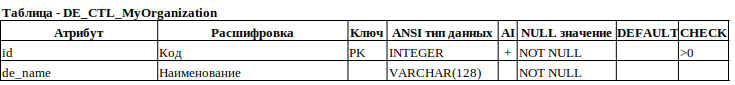
\includegraphics[width=18cm]
    {assets/database/Types/DE_CTL_MyOrganization.png}

    \caption{Таблица DE\_CTL\_MyOrganization}

    \label{fig:Logic_DE_CTL_MyOrganization}
\end{figure}

% = = = = = = = = = = = = = = = = = = = = = = = = = = = = = = = =

\subsubsection{Механизмы целостности для справочника <<Производители>>}

Таблица с механизмами целостности изображена на рисунке~\ref{fig:Logic_DE_CTL_Producers}.

\begin{figure}[!h]
    \centering

    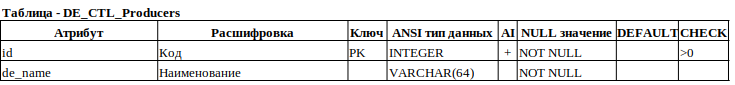
\includegraphics[width=18cm]
    {assets/database/Types/DE_CTL_Producers.png}

    \caption{Таблица DE\_CTL\_Producers}

    \label{fig:Logic_DE_CTL_Producers}
\end{figure}

% = = = = = = = = = = = = = = = = = = = = = = = = = = = = = = = =

\subsubsection{Механизмы целостности для справочника <<Местра хранения>>}

Таблица с механизмами целостности изображена на рисунке~\ref{fig:Logic_DE_CTL_StorageLocations}.

\begin{figure}[!h]
    \centering

    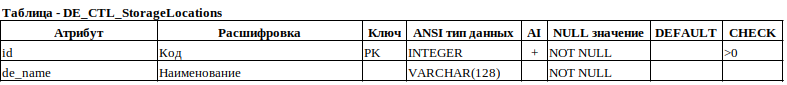
\includegraphics[width=18cm]
    {assets/database/Types/DE_CTL_StorageLocations.png}

    \caption{Таблица DE\_CTL\_StorageLocations}

    \label{fig:Logic_DE_CTL_StorageLocations}
\end{figure}

% = = = = = = = = = = = = = = = = = = = = = = = = = = = = = = = =

\subsubsection{Механизмы целостности для документа <<Приказ о создании комиссии>>}

Таблица с механизмами целостности изображена на рисунке~\ref{fig:Logic_DE_DOC_OrderCreationInventoryCommission}.

\begin{figure}[!h]
    \centering

    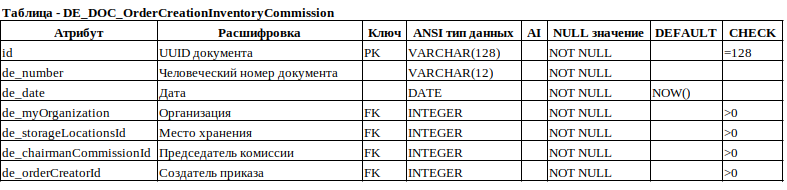
\includegraphics[width=18cm]
    {assets/database/Types/DE_DOC_OrderCreationInventoryCommission.png}

    \caption{Таблица DE\_DOC\_OrderCreationInventoryCommission}

    \label{fig:Logic_DE_DOC_OrderCreationInventoryCommission}
\end{figure}

% = = = = = = = = = = = = = = = = = = = = = = = = = = = = = = = =

\subsubsection{Механизмы целостности для документа <<Инвентаризационная опись>>}

Таблица с механизмами целостности изображена на рисунке~\ref{fig:Logic_DE_DOC_InventoryList}.

\begin{figure}[!h]
    \centering

    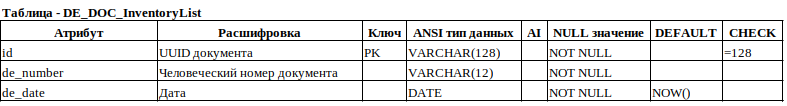
\includegraphics[width=18cm]
    {assets/database/Types/DE_DOC_InventoryList.png}

    \caption{Таблица DE\_DOC\_InventoryList}

    \label{fig:Logic_DE_DOC_InventoryList}
\end{figure}

% = = = = = = = = = = = = = = = = = = = = = = = = = = = = = = = =

\subsubsection{Механизмы целостности для табличной части <<Список членов комиссии>>}

Таблица с механизмами целостности изображена на рисунке~\ref{fig:Logic_DE_TAB_ListInventoryCommission}.

\begin{figure}[!h]
    \centering

    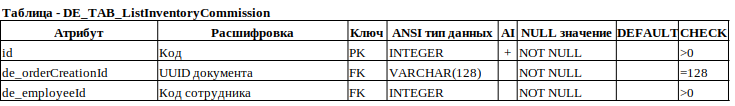
\includegraphics[width=18cm]
    {assets/database/Types/DE_TAB_ListInventoryCommission.png}

    \caption{Таблица DE\_TAB\_ListInventoryCommission}

    \label{fig:Logic_DE_TAB_ListInventoryCommission}
\end{figure}

% = = = = = = = = = = = = = = = = = = = = = = = = = = = = = = = =

\subsubsection{Механизмы целостности для табличной части <<Список номенклатуры инвентаризационной описи>>}

Таблица с механизмами целостности изображена на рисунке~\ref{fig:Logic_DE_TAB_NomenclatureInventList}.

\begin{figure}[!h]
    \centering

    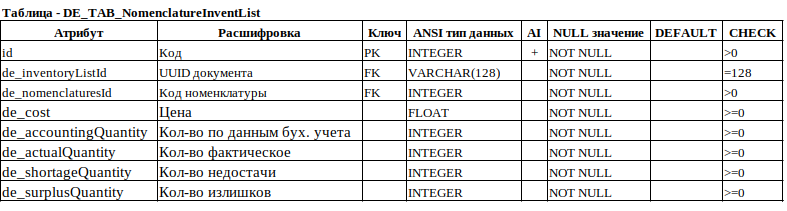
\includegraphics[width=18cm]
    {assets/database/Types/DE_TAB_NomenclatureInventList.png}

    \caption{Таблица DE\_TAB\_NomenclatureInventList}

    \label{fig:Logic_DE_TAB_NomenclatureInventList}
\end{figure}

% = = = = = = = = = = = = = = = = = = = = = = = = = = = = = = = =

\subsubsection{Проектирование логической модели}

Логическая модель доведенная до третьей нормальной формы,
спроектированная в SQL Power Architect 1.0.7 \cite{SqlPowerArhitect},
изображена на рисунке~\ref{fig:ArchitectureDatabase}.

\begin{figure}[!h]
    \centering

    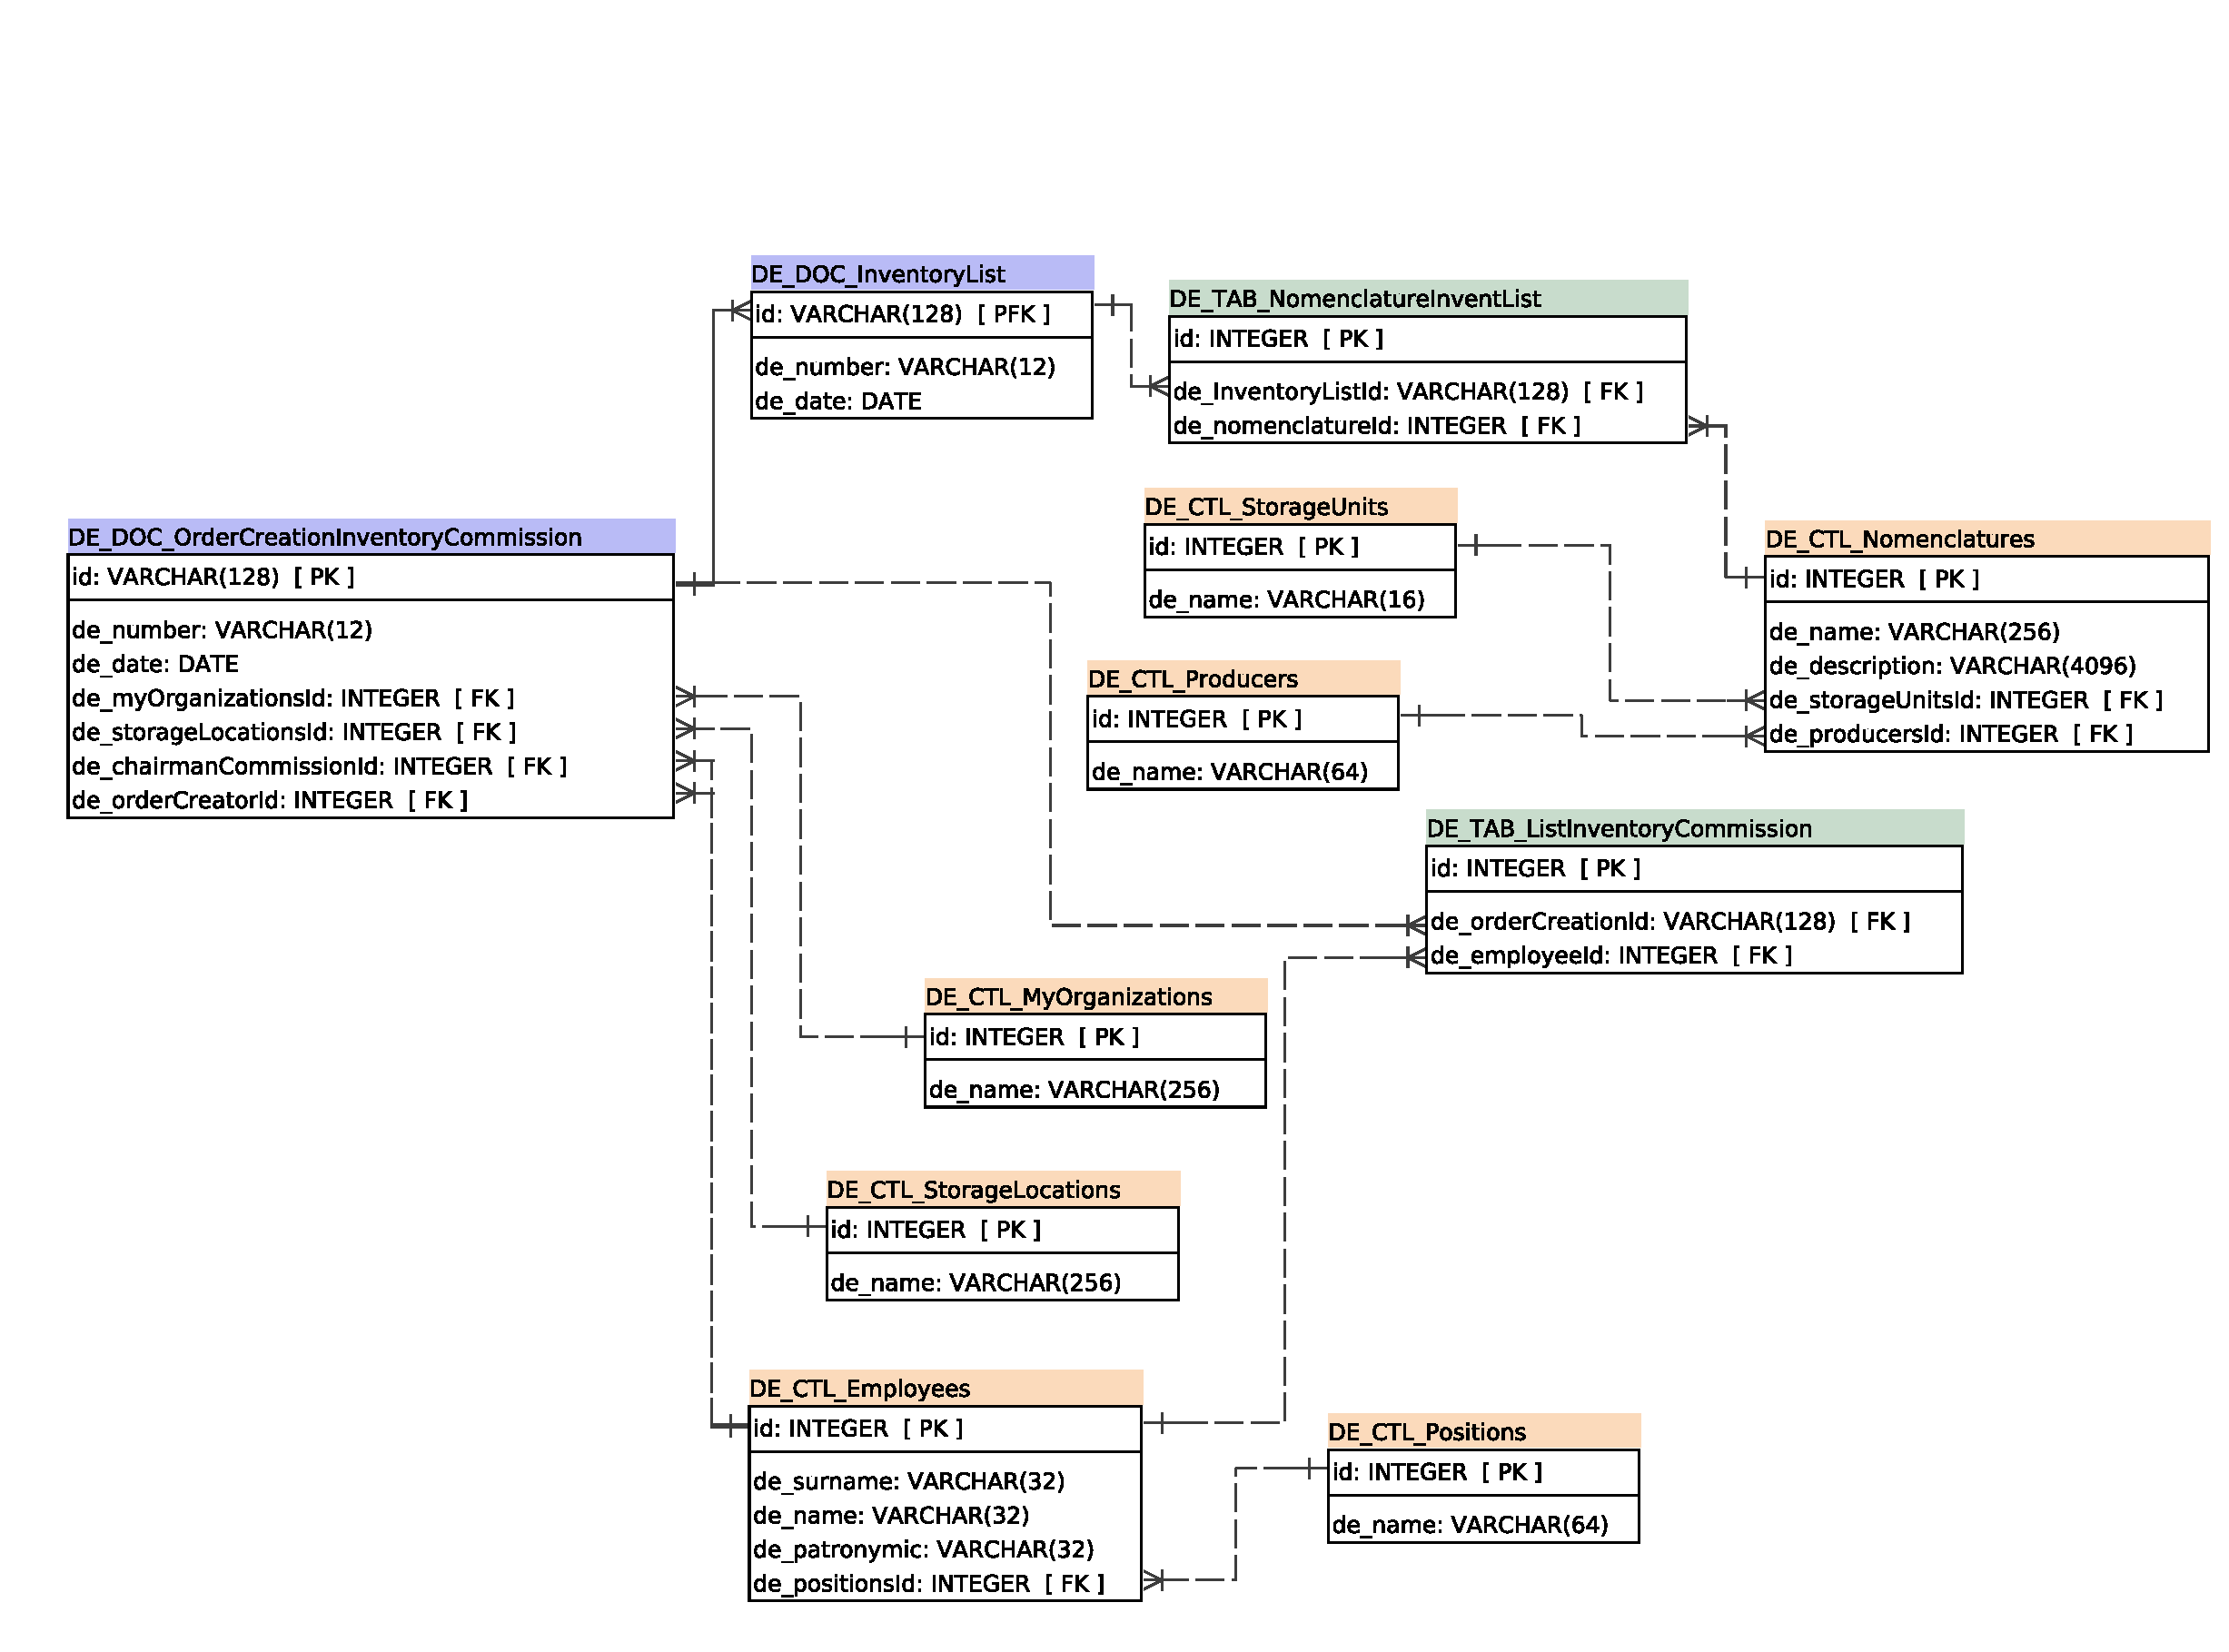
\includegraphics[width=17cm]
    {assets/database/LogicModel.SqlPowerArchitect.architect.pdf}

    \caption{Логическая модель}

    \label{fig:ArchitectureDatabase}
\end{figure}

\newpage
\subsection{Физическая модель}

\lstinputlisting[language=sql]
{assets/database/SQL_CreateTable.sql}

\newpage

\lstinputlisting[language=sql]
{assets/database/SQL_DropTable.sql}

\newpage
